%package list
\documentclass{article}
\usepackage[top=3cm, bottom=3cm, outer=3cm, inner=3cm]{geometry}
\usepackage{graphicx}
\usepackage{url}
%\usepackage{cite}
\usepackage{hyperref}
\usepackage{array}
\usepackage{multicol}
\newcolumntype{x}[1]{>{\centering\arraybackslash\hspace{0pt}}p{#1}}
\usepackage{natbib}
\usepackage{pdfpages}
\usepackage{multirow}
\usepackage{float}
\usepackage[normalem]{ulem}
\useunder{\uline}{\ul}{}


%%%%%%%%%%%%%%%%%%%%%%%%%%%%%%%%%%%%%%%%%%%%%%%%%%%%%%%%%%%%%%%%%%%%%%%%%%%%
%%%%%%%%%%%%%%%%%%%%%%%%%%%%%%%%%%%%%%%%%%%%%%%%%%%%%%%%%%%%%%%%%%%%%%%%%%%%
\newcommand{\csemail}{vmachacaa@unsa.edu.pe}
\newcommand{\csdocente}{Vicente Machaca Arceda}
\newcommand{\cscurso}{Estructura de Datos y Algoritmos}
\newcommand{\csuniversidad}{Universidad Nacional de San Agustín}
\newcommand{\csescuela}{Maestría en Ciencia de la Computación}
\newcommand{\cspracnr}{04}
\newcommand{\cstema}{--}
%%%%%%%%%%%%%%%%%%%%%%%%%%%%%%%%%%%%%%%%%%%%%%%%%%%%%%%%%%%%%%%%%%%%%%%%%%%%
%%%%%%%%%%%%%%%%%%%%%%%%%%%%%%%%%%%%%%%%%%%%%%%%%%%%%%%%%%%%%%%%%%%%%%%%%%%%


\usepackage[english,spanish]{babel}
\usepackage[utf8]{inputenc}
\AtBeginDocument{\selectlanguage{spanish}}
\renewcommand{\figurename}{Figura}
\renewcommand{\refname}{Referencias}
\renewcommand{\tablename}{Tabla} %esto no funciona cuando se usa babel
\AtBeginDocument{%
	\renewcommand\tablename{Tabla}
}

\usepackage{fancyhdr}
\pagestyle{fancy}
\fancyhf{}
\setlength{\headheight}{30pt}
\renewcommand{\headrulewidth}{1pt}
\renewcommand{\footrulewidth}{1pt}
\fancyhead[L]{\raisebox{-0.2\height}{
\includegraphics[width=3cm]{logo_unsa}}}

\fancyhead[C]{}
\fancyhead[R]{\fontsize{7}{7}\selectfont	\csuniversidad \\ \csescuela \\ \textbf{\cscurso} }
\fancyfoot[L]{MSc. Vicente Machaca}
\fancyfoot[C]{\cscurso}
\fancyfoot[R]{Página \thepage}







\begin{document}
	
	\vspace*{10px}
	
	\begin{center}	
		\fontsize{17}{17} \textbf{ Práctica \cspracnr}
	\end{center}
	%\centerline{\textbf{\underline{\Large Título: Informe de revisión del estado del arte}}}
	%\vspace*{0.5cm}
	

	\begin{table}[h]
		\begin{tabular}{|x{4.7cm}|x{4.8cm}|x{4.8cm}|}
			\hline 
			\textbf{DOCENTE} & \textbf{CARRERA}  & \textbf{CURSO}   \\
			\hline 
			\csdocente & \csescuela & \cscurso    \\
			\hline 
		\end{tabular}
	\end{table}	
	
	
	\begin{table}[h]
		\begin{tabular}{|x{4.7cm}|x{4.8cm}|x{4.8cm}|}
			\hline 
			\textbf{PRÁCTICA} & \textbf{TEMA}  & \textbf{DURACIÓN}   \\
			\hline 
			\cspracnr & \cstema & 3 horas   \\
			\hline 
		\end{tabular}
	\end{table}
	
	
	\section{Datos de los estudiantes}
	\begin{itemize}
		\item Grupo: 3
		\item Integrantes: 
		\begin{itemize}
			\item Lizarraga Mendoza David Jesus
			\item Saenz Mamani Alex Alberto
			\item Huaman Hilari Julissa Zaida
			\item Chara Condori Julio Cesar
			\item Acuña Chavez Melvin
		\end{itemize}		
	\end{itemize}
	
	
	

	
	\section{Trabajo de Investigación}\label{sec:ejercicios}
	\begin{enumerate}
		\item Clasificación de imágenes\\
		Para el presente  trabajo se utilizó un dataset de la siguiente fuente: 
		\url{https://www.kaggle.com/c/dogs-vs-cats/data}\\
		el cual representa un conjunto de imágenes de perros y gatos, alrededor de 2500 entre ambos.\\
		Este presente dataset se utilizará como base datos para entrenar al algoritmo de KNN, para la claificación entre las imágenes de gatos y perros.\\
		
	   
		\item Implementacion\\
		El aloritmo KNN que implementaremos se basa en las distancia entre vectores de punto a punto, para el cual utilizaremos la distancia euclidiana.\\
		EL algoritmo KNN clasifica los puntos encontrados más cercanos, de acuerdo a un vector de caracteristicas que se entreno previamente, el vector de caracteristicas que estamos tomando es un histograma de puntos de pixeles, el histograma busca puntos en una imagen el cual los junta y crea un descriptor.\\
		El descriptor toma los colores más oscuros de acuerdo al pelaje de un perro y para un gato seria un pelaje más fino, para ellos utilizamos una librería llamada "OpenCV", el cual permite el procesamiento de las imágenes del dataset que hemos elegido el cual genera el vector de caracteristicas del histograma.\\
		
		
\item Resultado\\
 El algoritmo KNN al momento de clasificar, enviamos una imagen de un gato o un perro como prueba el cual determinará el grado de parentesco pertenece de acuerdo a un porcentaje de exactitud.\\
 A continuación mostaremos los resultados obtenidos:\\
 
    \begin{enumerate}
        
        \item En la Figura 1 se muestra los resultados al 56.41 con el animal "Gato". \\\\
    
        \begin{figure1}
        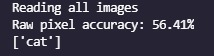
\includegraphics{result_1.jpeg}
        
        \caption{Figura 1: Resultado de parentesco "Gato".}
        \centering
        \end{figure1}\\
       
        
        %%%%COUNTING
        \item En la Figura 2, se muestra los resultados al 56.41 con el animal "Perro".\\\\
    
        \begin{figure2}
        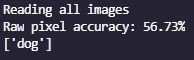
\includegraphics{result_2.jpeg}
        
        \caption{Figura 2: Resultado de parentesco "Perro".}
        \centering
        \end{figure2}\\
  
    \end{enumerate}
	 \item Video de Presentación\\
	 EL link de exposión de la práctica:\\
      \url{https://www.loom.com/share/bcb5dac057e04431af8fb8550b921e21}\\
      
      \item Ruta GitHub:\\
      \url{https://github.com/julissah/EDA-M/tree/development/EDA-M4}\\
	\end{enumerate}


	
	%\clearpage
	%\bibliographystyle{apalike}
	%\bibliographystyle{IEEEtranN}
	%\bibliography{bibliography}
	
	


		
	
\end{document}



		
	
\end{document}